\chapter{Proverb 11}

\begin{figure}
  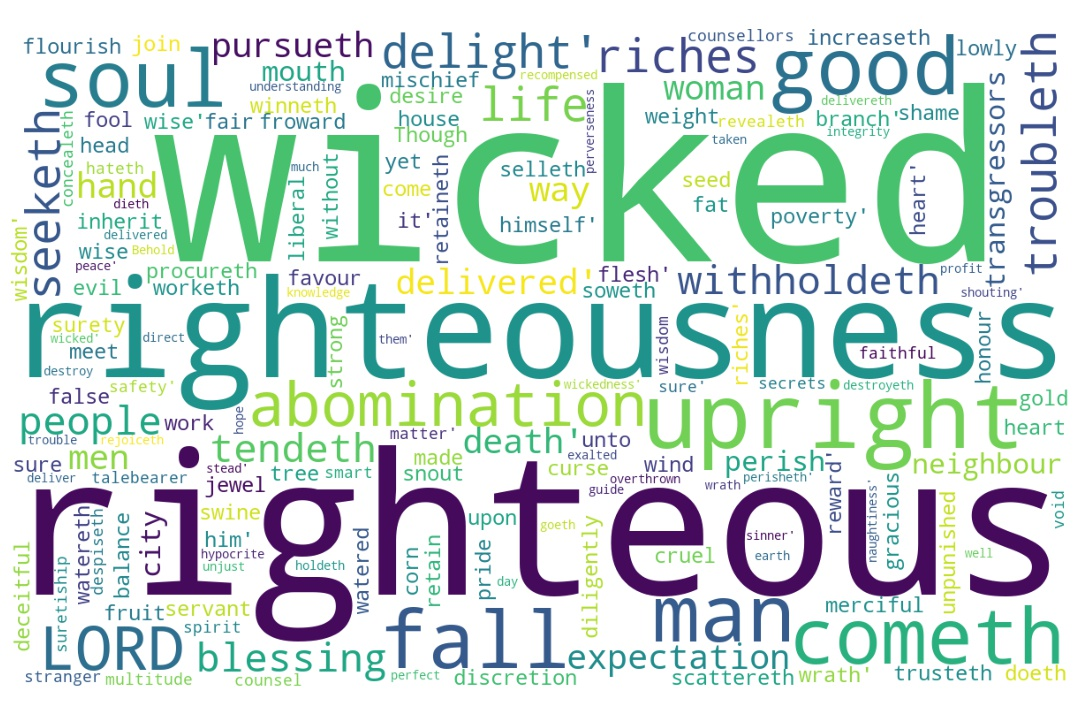
\includegraphics[width=\linewidth]{20OT-Proverbs/Proverb11-WordCloud.jpg}
  \caption{Proverb 11 Word Cloud}
  \label{fig:Proverb 11 Word Cloud}
\end{figure}

\marginpar{\scriptsize \centering \fcolorbox{bone}{lime}{\textbf{MISSING IMPORTANT THINGS}}\\ (Proverbs 11:1-31) \begin{compactenum}[I.][8]
    \item No \textbf{Balance} \index[scripture]{Proverbs!Pro 11:01} (Pro 11:1) 
    \item No \textbf{Integrity} \index[scripture]{Proverbs!Pro 11:03}(Pro 11:3) 
    \item No \textbf{Expectation} \index[scripture]{Proverbs!Pro 11:07}(Pro 11:7) 
    \item No \textbf{Wisdom} \index[scripture]{Proverbs!Pro 11:12}(Pro 11:12) 
    \item No \textbf{Counsel} \index[scripture]{Proverbs!Pro 11:14}(Pro 11:14) 
    \item No \textbf{Discretion} \index[scripture]{Proverbs!Pro 11:22}(Pro 11:22) 
    \item No \textbf{Corn (food)} \index[scripture]{Proverbs!Pro 11:26}(Pro 11:26) 
\end{compactenum}}

\marginpar{\scriptsize \centering \fcolorbox{bone}{yellow}{\textbf{UNDEPENDABLE}}\\ (Proverbs 11:1-31) \begin{compactenum}[I.][8]
    \item \textbf{Riches in the Day of Wrath} \index[scripture]{Proverbs!Pro 11:04}\index[scripture]{Proverbs!Pro 11:28}(Pro 11:4, 28)
    \item \textbf{A Hypocrite to Keep his Word} \index[scripture]{Proverbs!Pro 11:09}(Pro 11:9)
    \item \textbf{Mouth of the Wicked}\index[scripture]{Proverbs!Pro 11:11} (Pro 11:11)
    \item \textbf{A Foolish Neighbor Providing Wisdom} \index[scripture]{Proverbs!Pro 11:12}(Pro 11:12)
    \item \textbf{Lasting Blessing from a Deceitful Work} \index[scripture]{Proverbs!Pro 11:18}(Pro 11:18)
    \item \textbf{Discretion from an Evil Woman} \index[scripture]{Proverbs!Pro 11:22} (Pro 11:22)
    \item \textbf{A Fool to not Withhold}\index[scripture]{Proverbs!Pro 11:24}\index[scripture]{Proverbs!Pro 11:27} (Pro 11:24, 27)
\end{compactenum}}

\marginpar{\scriptsize \centering \fcolorbox{bone}{black}{\textbf{\textcolor[cmyk]{0,0,0,0}{WALKING THE RIGHT PATH}}}\\ (Proverbs 11) \begin{compactenum}[I.][8]
    \item The \textbf{Delight of the Lord} \index[scripture]{Proverbs!Pro 11:01}\index[scripture]{Proverbs!Pro 11:20}(Pro 11:1, 20)
     \item   \textbf{Deliverance} \index[scripture]{Proverbs!Pro 11:04}  \index[scripture]{Proverbs!Pro 11:06} \index[scripture]{Proverbs!Pro 11:08} \index[scripture]{Proverbs!Pro 11:09} \index[scripture]{Proverbs!Pro 11:21}(Pro 11:4, 6, 8, 9, 21)
     \item  A \textbf{Directing} \index[scripture]{Proverbs!Pro 11:05} (Pro 11:5)
   \item  \textbf{Discretion} \index[scripture]{Proverbs!Pro 11:22} (Pro 11:22)
   \item  \textbf{Desire} \index[scripture]{Proverbs!Pro 11:23} (Pro 11:23)
   \item  \textbf{Diligence} \index[scripture]{Proverbs!Pro 11:27} (Pro 11:27)
    \item  A \textbf{Destination} \index[scripture]{Proverbs!Pro 11:30} (Pro 11:30)
\end{compactenum}}

\marginpar{\scriptsize \centering 
\fcolorbox{black}{blue}{\textbf{\textcolor[cmyk]{0,0,0,0}{A PERSON OUT OF BALANCE}}}\\ 
(Proverbs 11:1) 
\begin{compactenum}[I.][8]
    \item \textbf{Tends to Fall a Lot}  
    \item \textbf{Breaks Things}
    \item \textbf{Bumps Into Things}  
    \item \textbf{Looks Funny or Foolish or Pathetic}
    \item \textbf{Usually Needs a Crutch}
    \item \textbf{Requires Extra Attention}
    \item \textbf{Throws off Judgment}
\end{compactenum}}




\footnote{\textcolor[cmyk]{0.99998,1,0,0}{\hyperlink{TOC}{Return to end of Table of Contents.}}}\footnote{\href{https://www.audioverse.org/english/audiobibles/books/ENGKJV/O/Prov/1}{\textcolor[cmyk]{0.99998,1,0,0}{Proverbs Audio}}}\textcolor[cmyk]{0.99998,1,0,0}{A \fcolorbox{bone}{lime}{false balance} \emph{is} abomination to the LORD: but \fcolorbox{bone}{bone}{a} just weight \emph{is} \fcolorbox{bone}{bone}{his} delight.}\footnote{\textbf{Proverb 16:11} - A just weight and balance are the LORD's: all the weights of the bag are his work.}\footnote{\textbf{Proverb 20:10} - Divers weights, and divers measures, both of them are alike abomination to the LORD.}\footnote{\textbf{Proverb 20:23} - Divers weights are an abomination unto the LORD; and a false balance is not good.}\footnote{\textbf{Ezekiel 45:10-12} - Ye shall have just balances, and a just ephah, and a just bath. [11] The ephah and the bath shall be of one measure, that the bath may contain the tenth part of an homer, and the ephah the tenth part of an homer: the measure thereof shall be after the homer. [12] And the shekel shall be twenty gerahs: twenty shekels, five and twenty shekels, fifteen shekels, shall be your maneh.}\footnote{\textbf{Hosea 12:7} - He is a merchant, the balances of deceit are in his hand: he loveth to oppress.}\footnote{\textbf{Amos 8:5-6} - Saying, When will the new moon be gone, that we may sell corn? and the sabbath, that we may set forth wheat, making the ephah small, and the shekel great, and falsifying the balances by deceit? That we may buy the poor for silver, and the needy for a pair of shoes; yea, and sell the refuse of the wheat?}\footnote{\textbf{Micah 6:10-11} - Are there yet the treasures of wickedness in the house of the wicked, and the scant measure that is abominable? Shall I count them pure with the wicked balances, and with the bag of deceitful weights?}
[2] \textcolor[cmyk]{0.99998,1,0,0}{\emph{When} pride cometh, then cometh shame: but with the lowly \emph{is} wisdom.}\footnote{\textbf{Proverb 16:18-19} - Pride goeth before destruction, and an haughty spirit before a fall. [19] Better it is to be of an humble spirit with the lowly, than to divide the spoil with the proud.}\footnote{\textbf{Daniel 4:30-32} - The king spake, and said, Is not this great Babylon, that I have built for the house of the kingdom by the might of my power, and for the honour of my majesty? [31] While the word was in the king's mouth, there fell a voice from heaven, saying, O king Nebuchadnezzar, to thee it is spoken; The kingdom is departed from thee. [32] And they shall drive thee from men, and thy dwelling shall be with the beasts of the field: they shall make thee to eat grass as oxen, and seven times shall pass over thee, until thou know that the most High ruleth in the kingdom of men, and giveth it to whomsoever he will.}\footnote{\textbf{Proverb 15:33} - The fear of the LORD is the instruction of wisdom; and before honour is humility.}\footnote{\textbf{1 Corinthians 8:1-2} - Now as touching things offered unto idols, we know that we all have knowledge. Knowledge puffeth up, but charity edifieth. [2] And if any man think that he knoweth any thing, he knoweth nothing yet as he ought to know.}
[3] \textcolor[cmyk]{0.99998,1,0,0}{The \fcolorbox{bone}{lime}{integrity} of the upright shall guide them: but the perverseness of \fcolorbox{bone}{MYGOLD}{transgressors} shall destroy them.}
[4] \textcolor[cmyk]{0.99998,1,0,0}{Riches profit not in the day of wrath: but \fcolorbox{bone}{MYGOLD}{righteousness} delivereth from death.}
[5] \textcolor[cmyk]{0.99998,1,0,0}{The \fcolorbox{bone}{MYGOLD}{righteousness} of the perfect shall direct \fcolorbox{bone}{bone}{his} way: but the wicked shall fall by \fcolorbox{bone}{bone}{his} own wickedness.}
[6] \textcolor[cmyk]{0.99998,1,0,0}{The \fcolorbox{bone}{MYGOLD}{righteousness} of the upright shall deliver them: but \fcolorbox{bone}{MYGOLD}{transgressors} shall be taken in \emph{their} \emph{own} naughtiness.}
[7] \textcolor[cmyk]{0.99998,1,0,0}{When \fcolorbox{bone}{bone}{a} wicked man dieth, \emph{his} \fcolorbox{bone}{lime}{expectation} shall perish: and the hope of unjust \emph{men} perisheth.}
[8] \textcolor[cmyk]{0.99998,1,0,0}{The righteous is delivered out of trouble, and the wicked cometh in \fcolorbox{bone}{bone}{his} stead.}
[9] \textcolor[cmyk]{0.99998,1,0,0}{An hypocrite with \emph{his} mouth destroyeth \fcolorbox{bone}{bone}{his} neighbour: but through knowledge shall the just be delivered.}
[10] \textcolor[cmyk]{0.99998,1,0,0}{When it goeth well with the righteous, the city rejoiceth: and when the wicked perish, \emph{there} \emph{is} shouting.}
[11] \textcolor[cmyk]{0.99998,1,0,0}{By the blessing of the upright the city is exalted: but it is overthrown by the mouth of the wicked.}
[12] \textcolor[cmyk]{0.99998,1,0,0}{He that is void of \fcolorbox{bone}{lime}{wisdom} despiseth \fcolorbox{bone}{bone}{his} neighbour: but \fcolorbox{bone}{bone}{a} man of \fcolorbox{bone}{MYGOLD}{understanding} holdeth \fcolorbox{bone}{bone}{his} peace.}
[13] \textcolor[cmyk]{0.99998,1,0,0}{A talebearer revealeth secrets: but he that is of \fcolorbox{bone}{bone}{a} faithful spirit concealeth the matter.}
[14] \textcolor[cmyk]{0.99998,1,0,0}{Where \fcolorbox{bone}{lime}{no counsel} \emph{is}, the people fall: but in the multitude of counsellors \emph{there} \emph{is} safety.}\footnote{\textbf{Proverb 15:22} - Without counsel purposes are disappointed: but in the multitude of counsellors they are established.}\footnote{\textbf{Proverb 16:22} - Understanding is a wellspring of life unto him that hath it: but the instruction of fools is folly.}\footnote{\textbf{Proverb 24:6} - For by wise counsel thou shalt make thy war: and in multitude of counsellors there is safety.}
[15] \textcolor[cmyk]{0.99998,1,0,0}{He that is surety for \fcolorbox{bone}{bone}{a} stranger shall smart \emph{for} \emph{it}: and he that hateth suretiship is sure.}\footnote{\textbf{Proverb 6:1-5} - My son, if thou be surety for thy friend, if thou hast stricken thy hand with a stranger, [2] Thou art snared with the words of thy mouth, thou art taken with the words of thy mouth. [3] Do this now, my son, and deliver thyself, when thou art come into the hand of thy friend; go, humble thyself, and make sure thy friend. [4] Give not sleep to thine eyes, nor slumber to thine eyelids. [5] Deliver thyself as a roe from the hand of the hunter, and as a bird from the hand of the fowler.}
[16] \textcolor[cmyk]{0.99998,1,0,0}{A gracious woman retaineth honour: and strong \emph{men} retain riches.}
[17] \textcolor[cmyk]{0.99998,1,0,0}{The merciful man doeth good to \fcolorbox{bone}{bone}{his} own soul: but \emph{he} \emph{that} \emph{is} cruel troubleth \fcolorbox{bone}{bone}{his} own flesh.}
[18] \textcolor[cmyk]{0.99998,1,0,0}{The wicked worketh \fcolorbox{bone}{bone}{a} deceitful work: but to him that soweth \fcolorbox{bone}{MYGOLD}{righteousness} \emph{shall} \emph{be} \fcolorbox{bone}{bone}{a} sure reward.}
[19] \textcolor[cmyk]{0.99998,1,0,0}{As \fcolorbox{bone}{MYGOLD}{righteousness} \emph{tendeth} to life: so he that pursueth evil \emph{pursueth} \emph{it} to \fcolorbox{bone}{bone}{his} own death.}
[20] \textcolor[cmyk]{0.99998,1,0,0}{They that are of \fcolorbox{bone}{bone}{a} froward heart \emph{are} abomination to the LORD: but \emph{such} \emph{as} \emph{are} upright in \emph{their} way \emph{are} \fcolorbox{bone}{bone}{his} delight.}
[21] \textcolor[cmyk]{0.99998,1,0,0}{\emph{Though} hand \emph{join} in hand, the wicked shall not be unpunished: but the seed of the righteous shall be delivered.}
[22] \textcolor[cmyk]{0.99998,1,0,0}{\emph{As} a jewel of gold in \fcolorbox{bone}{bone}{a} swine's snout, \emph{so} \emph{is} \fcolorbox{bone}{bone}{a} fair woman which is without \fcolorbox{bone}{lime}{discretion}.}
[23] \textcolor[cmyk]{0.99998,1,0,0}{The desire of the righteous \emph{is} only good: \emph{but} the expectation of the wicked \emph{is} wrath.}
[24] \textcolor[cmyk]{0.99998,1,0,0}{There is that scattereth, and yet increaseth; and \emph{there} \emph{is} that withholdeth more than is meet, but \emph{it} \emph{tendeth} to poverty.}
[25] \textcolor[cmyk]{0.99998,1,0,0}{The liberal soul shall be made fat: and he that watereth shall be watered also himself.}
[26] \textcolor[cmyk]{0.99998,1,0,0}{He that \fcolorbox{bone}{lime}{withholdeth corn}, the people shall curse him: but blessing \emph{shall} \emph{be} upon the head of him that selleth \emph{it}.}
[27] \textcolor[cmyk]{0.99998,1,0,0}{He that diligently seeketh good procureth favour: but he that seeketh mischief, it shall come unto him.}
[28] \textcolor[cmyk]{0.99998,1,0,0}{He that trusteth in \fcolorbox{bone}{bone}{his} riches shall fall: but the righteous shall flourish as \fcolorbox{bone}{bone}{a} branch.}
[29] \textcolor[cmyk]{0.99998,1,0,0}{He that troubleth \fcolorbox{bone}{bone}{his} own house shall inherit the wind: and the fool \emph{shall} \emph{be} servant to the wise of heart.}\footnote{\textbf{1 Samuel 25:3, 17, 38} - Now the name of the man was Nabal; and the name of his wife Abigail: and she was a woman of good understanding, and of a beautiful countenance: but the man was churlish and evil in his doings; and he was of the house of Caleb. [17] Now therefore know and consider what thou wilt do; for evil is determined against our master, and against all his household: for he is such a son of Belial, that a man cannot speak to him. [38] And it came to pass about ten days after, that the LORD smote Nabal, that he died.}\footnote{\textbf{Hosea 8:7} - For they have sown the wind, and they shall reap the whirlwind: it hath no stalk: the bud shall yield no meal: if so be it yield, the strangers shall swallow it up.}
[30] \textcolor[cmyk]{0.99998,1,0,0}{The fruit of the righteous \emph{is} \fcolorbox{bone}{bone}{a} tree of life; and he that winneth souls \emph{is} wise.}\footnote{\textbf{Proverb 3:18} - She is a tree of life to them that lay hold upon her: and happy is every one that retaineth her.}\footnote{\textbf{Proverb 15:4} -A wholesome tongue is a tree of life: but perverseness therein is a breach in the spirit.}\footnote{\textbf{Daniel 12:3} - And they that be wise shall shine as the brightness of the firmament; and they that turn many to righteousness as the stars for ever and ever.}\footnote{\textbf{James 5:20} - Let him know, that he which converteth the sinner from the error of his way shall save a soul from death, and shall hide a multitude of sins.}
[31] \textcolor[cmyk]{0.99998,1,0,0}{Behold, the righteous shall be recompensed in the earth: much more the wicked and the sinner.}
